%%%%%%%%%%%%%%%%%%%%%%%%%%%%%%%%%%%%%%%%%%%%%%%%%%%%%%%%%%%%%%%%%%%%%%%%%%closed-loop%%%%%%%%%%%%%%%%%%%%%%%%%
\documentclass[letterpaper, 10 pt, journal, twocolumn]{IEEEtran}  % Comment this line out
                                                          % if you need a4paper
%\documentclass[a4paper, 10pt, conference]{ieeeconf}      % Use this line for a4
                                                          % paper

%\IEEEoverridecommandlockouts                              % This command is only
                                                          % needed if you want to
                                                          % use the \thanks command
%\overrideIEEEmargins
% See the \addtolength command later in the file to balance the column lengths
% on the last page of the document
%\usepackage[T1]{fontenc}
%\usepackage[latin1]{inputenc}
%
%%%%%%%%%%%%%%%%%%%%%%%%%%%%%%%%%%%%%%%%%%%%%%%%%%%
\usepackage{graphics} % for pdf, bitmapped graphics files
\usepackage{epsfig} % for postscript graphics files
\usepackage{mathptmx} % assumes new font selection scheme installed
\usepackage{times} % assumes new font selection scheme installed
\usepackage{amsmath} % assumes amsmath package installed
\usepackage{amssymb}  % assumes amsmath package installed
%%%%%%%%%%%%%%%%%%%%%%%%%%%%%%%%%%%%%%%%%%%%%%%%%%%
%\usepackage{lmodern}
\usepackage{graphics} % for pdf, bitmapped graphics files
\usepackage{graphicx}     % 
\usepackage{color}
\usepackage{xcolor}
\usepackage{epsfig} % for postscript graphics files
\usepackage{epstopdf}     % conversion to .pdf
\usepackage{url}
\usepackage{calc}
\usepackage{float}
\usepackage{siunitx}
\usepackage{xspace}
\usepackage{standalone}
\usepackage{comment}
\let\proof\relax 
\let\endproof\relax 
\usepackage{amsthm}
\let\labelindent\relax
\usepackage{enumitem}
%%%%%%%%%%%%%%%%%%%%%%%%%%%%%%%%%%%%%%%%%%%%%%%%%%%
\usepackage{tikz}
\usetikzlibrary{positioning,arrows}
%%%%%%%%%%%%%%%%%%%%%%%%%%%%%%%%%%%%%%%%%%%%%%%%%%%

%%%%%%%%%%%%%%%%%%%%%%%%%%%%%%%%%%%%%%%%%%%%%%%%%%%
\usepackage{cite}
\bibliographystyle{IEEEtran}
%
\usepackage{hyperref}
\hypersetup{plainpages = {false},
			bookmarksopen = {true},
			bookmarksnumbered = {true},
			breaklinks = {true},
			pdfstartview={FitH},
			pdfcreator={PDFtime-varyingLaTeX-DPD},	
			pdfproducer={PDFLaTeX-DPD},	
			colorlinks=true,
			citecolor=black,
			linkcolor=black,
			urlcolor=black,
			filecolor=black,
			bookmarksopen=true
} % links em preto
%%%%%%%%%%%%%%%%%%%%%%%%%%%%%%%%%%%%%%%%%%%%%%%%%%%
% Graphical path
\graphicspath{{./Figs/}}
%%%%%%%%%%%%%%%%%%%%%%%%%%%%%%%%%%%%%%%%%%%%%%%%%%%
% TIKZ % ---
% Defining string as labels of certain blocks.
\newcommand{\suma}{\Large$+$}
\newcommand{\sumb}{\Large$\Sigma$}
\newcommand{\minusa}{\Large$-$}
\newcommand{\timesa}{\Large$\times$}
\newcommand{\inte}{$\displaystyle \int$}
\newcommand{\derv}{\huge$\frac{d}{dt}$}

\newcommand{\dd}[1]{ %Marca uma revis�o
    {\color{red}[\![} {\color{blue}\bf#1\xspace} {\color{red}]\!]}
}
\def\re{{\rm I}\! {\rm R}}
\newcommand{\mref}[1]{(\ref{#1})}
\newcommand{\sat}[1]{\mbox{sat}\,}
\renewcommand{\t}{^{\mbox{\tiny\sf T}}} % transposto 
\newcommand\norm[1]{\ensuremath{\lVert#1\rVert}}
\newcommand\abs[1]{\ensuremath{\lvert#1\rvert}}
\newcommand{\matx}[1]{{\textbf #1}}
\def\QED{\mbox{\rule[0pt]{1.0ex}{1.0ex}}} 
\def\proof{\noindent\hspace{2em}{\it Proof: }}
\def\endproof{\hspace*{\fill}~\QED\par\endtrivlist\unskip}
%
\newcommand{\rd}[1]{\textcolor{red}{#1}}
\newcommand{\unit}[1]{\si{#1}}
\newcommand{\myunit}[2]{\num{#1}\,\si{#2}}
%----------------------------------------------------
%  Cross references
%----------------------------------------------------
\newcommand{\tabref}[1]{Tabela~\ref{#1}}
\renewcommand{\eqref}[1]{Eq.~(\ref{#1})}
\newcommand{\figref}[1]{Fig.~\ref{#1}}
\newcommand{\figuref}[1]{Figure~\ref{#1}}
\newcommand\scalemath[2]{\scalebox{#1}{\mbox{\ensuremath{\displaystyle #2}}}}
\setlength{\abovecaptionskip}{0pt}
\setlength{\belowcaptionskip}{-10pt} % reduce space
%%%%%%%%%%%%%%%%%%%%%%%%%%%%%%%%%%%%%%%%%%%%%%%%%%%
%
\theoremstyle{plain}
\newtheorem{theorem}{Theorem}
\newtheorem{lemma}[theorem]{Lemma}
\newtheorem{prop}[theorem]{Proposition}
\newtheorem*{cor}{Corollary}
%
\theoremstyle{definition}
\newtheorem{defn}{Definition}
\newtheorem{conj}{Conjecture}
\newtheorem{exmp}{Example}
%
\theoremstyle{remark}
\newtheorem*{remark}{Remark}
\newtheorem*{note}{Note}
%%%%%%%%%%%%%%%%%%%%%%%%%%%%%%%%%%%%%%%%%%%%%%%%%%%
%
\title{\LARGE \bf
Smooth Sliding Control Applied to Prosthetic Legs via Variable High Gain Observer}


\author{Alessandro J. Peixoto, %
        Ign\'{a}cio de A. M. Ricart and
        Matheus Ferreira dos Reis %and
		%Diego Pereira Dias%		 <-this % stops a space
		%
% <-this % stops a space
}

%%
%%%%%%%%%%%%%%%%%%%%%%%%%%%%%%%%%%%%%%%%%%%%%%%%%%%%%
\begin{document}
%\onecolumn

%%%%%%%%%%%%%%%%%%%%%%%%%%%%%%%%%%%%%%%%%%%%%%%%%%%%%
\DeclareGraphicsExtensions{.pdf,.png,.jpg,.jpeg,.mps,.ps,.eps}
\maketitle
\thispagestyle{empty}
\pagestyle{empty}
%%%%%%%%%%%%%%%%%%%%%%%%%%%%%%%%%%%%%%%%%%%%%%%%%%%%%
\begin{abstract}%
This draft focus on state estimation and control of a robot/prosthesis control system with four joints: vertical hip displacement, thigh, knee and ankle angles. The motivation was inspired by several drawbacks regarding the usage of load cells and/or sensors in robots and prosthetic legs to capture gait data, external forces (GRFs) and moments during walking. Thus, state estimation via Extended Kalman Filter (EKF), High-gain-observer (HGO) and Sliding Mode Observer (SMO) are promising as well as the estimation of forces acting on the prosthetic foot. We propose the implementation of an HGO with variable dynamic gain. The key idea is to design a time-varying HGO gain synthesized from measurable signals. This dynamic gain can be designed to: (i) reduce the amount of noise in the control signal while keeping an acceptable tracking error  transient performance; (ii) guarantee global/semi-global stability properties of the closed-loop system. The main focus is given to the HGO design while the smooth sliding control scheme is left for a future draft of this note. 
\end{abstract}
%%%
%%%\keywords{Smooth sliding mode control, extremum seeking control, wind power generation.}
%=============================================================
% INTRODUCTION
%%%%%%%%%%%%%%%%%%%%%%%%%%%%%%%%%%%%%%%%%%%%%%%%%%%%%%%%%%%%%%%%%%%%%%%%%%%%%%%%
\section{Introduction}

Prosthesis are devices that substitute the function of a missing limb either due to amputation or a congenital defect. Amputations could occur due to injuries, circulatory and vascular disease, diabetes or cancer and that means a huge number of people that could maintain their activities of daily livings (ADLs) and have the mobility partially / completely restored through improvements in prosthesis technology. 

There are three main types of prosthesis currently available: purely passive, active-damping controlled and powered controlled prostheses. The first type requires a significant effort from the amputee because there are only passive mechanical systems to assist him during the gait. Active damping uses microprocessors and sensors to measure when knee flexion and extension is needed based on encoder measures and load transfer acquired from observer/load cells. In this way, it can actively regulate the prosthesis damping factor and help the user during stance phases and during the gait.

A powered controlled prosthesis requires less metabolic energy from the user for walking than purely passive because they are able to generate net power at the joints through DC Motors or pneumatic actuators (ref-Design of a pneumatically actuated transfemoral prosthesis and Actuated leg prosthesis for above knee amputees and Towards a Smart semi-active prosthetic leg preliminary assessment and testing). As they are able to supply positive power, the user could more easily realize tasks such as climbing stairs, walking uphill.

The sensors applied to this type of prosthesis measure the joint angles such as high-resolution rotary encoders and forces such as strain gauges or load cells. Angular velocities could be acquired through expensive tacometers or numerical differentiation. Usually the numerical approach is applied using observers, which have to deal with the challenges of noise rejection.  

In the present paper, a proportional-integral-derivative (PID) control method is developed in order to make a robotic prosthetic leg follow a desired walking pattern. A feedback loop, using computed torque, is designed to linearize the plant and an HGO with variable gain is applied to estimate each joint angular velocity. 

Output-feedback control strategies using HGOs \cite{OK:97}
represent an important design class, in particular those schemes based on time-varying high gain
techniques (HGO with variable gain) \cite{P:01}\cite{KKJ:02}
\cite{KKC:03}\cite{LL:05}\cite{AK:07}.

In \cite{POH:2011}, \cite{PHCL:2007}, an output-feedback sliding-mode control design have been proposed for arbitrary relative
degree uncertain systems, where the class of plants encompasses time-varying minimum phase nonlinear plants, affine
in the control, transformable to a normal form and for which a
norm state estimator can be implemented. The main objective in \cite{POH:2011} was to use a dynamic observer gain in order to obtain global results without invoking the global Lipschitz-like restrictions. 

In addition, time-varying HGOs have also been used to cope with the effect of
measurement noise and to establish the connections with the
Extended Kalman Filter \cite{AK:07}\cite{AK:09}.

Considering that the present system has parametric uncertainties and angle measurement is subject to noise, a time-varying HGO design is proposed, similar to \cite{POH:2011}. While estimating in real-time the control signal noise, the adaptation law changes the observer gain to achieve a preferable trade-off between control noise and tracking performance. Global results are not pursued in this paper.

This variable gain approach is different from most of the existing techniques,
where the HGO gain is updated either solving a Riccati equation
\cite{P:01}\cite{P:07}\cite{GAL:06} or via 
functions based on measurable signals and norm
domination techniques \cite{LL:05}, \cite{P:07}, \cite{APA:09} and \cite{POH:2011}.

The proposed approach is verified in a simulation environment with a 4-link robot/prosthesis system (PRRR), with parameters extracted from \cite{Richter2015}. The human gait used as reference signal is obtained from \cite{Schwartz2008}.

This paper is organized as follows. In Section \ref{sec:System_model}, the system model is described where some considerations regarding the HGO design are taken into. Section \ref{sec:HGO} presents the HGO structure and the adapting function used in simulation. Section \ref{sec:Numerical_Simulation} shows the control law applied to the plant and results obtained. Finally, Section \ref{sec:Conclusions} presents concluding remarks and future work.

\section{Preliminaries}


The following notations and terminology are used:% in the paper:


%\subsection{Notation and Terminology}

%Let $[0,t_M)$ be the maximal time interval of definition of a
%given (plant or controller) solution of system
%(\ref{eq:planta_state}), where $t_M$ may be finite or infinite.
%For any $t_*\!\in\![0,t_M)$ let $\mathcal{I}\!:=\![t_*,t_M)$.

\begin{itemize}

\item The 2-norm (Euclidean) of a vector $x$ and the corresponding
induced norm of a matrix $A$ are denoted by $|x|$ and $|A|$,
respectively. The symbol $\lambda[A]$ denotes the spectrum of $A$
and $\lambda_m[A]=-\max_i\{Re\{\lambda[A]\}\}$.


\item The ${\mathcal{L}}_{\infty e}$ norm of a signal
$x(t)\!\in\!\re^n$ is defined as
$\|x_{t}\|\!:=\!\sup_{0\!\leq\!\tau\!\leq\!t} |x(\tau)|$.


\item  The symbol  ``$s$'' represents either the
Laplace variable or the differential operator ``$d/dt$'', according
to the context. 

\item As in \cite{IS:96} the output $y$ of a linear time invariant (LTI) system with transfer function
$H(s)$ and input $u$ is given by $y=H(s)u$. Convolution operations $h(t)*u(t)$, with $h(t)$ being the impulse response from $H(s)$, will be eventually written, for simplicity, as $H(s)*u$.


\item Classes of $\mathcal{K}, \mathcal{K}_\infty$ functions are
defined according to \cite[p.~144]{K:02}. ISS, OSS and IOSS mean
Input-State-Stable (or Stability), Output-State-Stable (or
Stability) and Input-Output-State-Stable, respectively
\cite{SW:95}.


\item The symbol $\pi$ denotes class-$\mathcal{KL}$ functions. Eventually, we denote by $\pi (t)$ any exponentially decreasing signal, i.e., a signal satisfying $|\pi(t)| \leq \Pi(t)$, where $\Pi(t):=R e^{-\lambda t}$, $\forall t$, for  some scalars $R,\lambda>0$.
\end{itemize}

%%%%%%%%%%%%%%%%%%%%%%%%%%%%%%%%%%%%%%%%%%%%%%%%%%%%%%%%%%%%%%%%%%%%%%%%%

\section{System Model}
\label{sec:System_model}

The dynamics of the machine/prosthesis system composed by a $4$-link rigid body robot\footnote{A more general framework with a $n$-link rigid body robot can also be considered. However, in order to keep this note close to \cite{Richter2015}, for simplicity, we have set $n=4$.}  with prismatic-revolute-revolute-revolute (PRRR) configuration, following the notation in \cite{Richter2015}, is given by:
%
\begin{equation}
D(q)\ddot{q} + C(q,\dot{q})\dot{q}+B(q,\dot{q}) + P(\dot{q}) + J_e^T F_e+g(q) = F_a\,,
\label{eq:Dinamica}
\end{equation}
%
where  $q$ represents the vector of joints positions ($q_1$ represents the hip vertical displacement, $q_2$ is the thigh angle, $q_3$ is the knee angle and $q_4$ represents ankle angle), $D(q)$ is the inertia matrix, $C(q,\dot{q})$ is the matrix of Coriolis and centrifugal forces, $B(q,\dot{q})$ is the knee  damper nonlinear matrix, $J_e$ is the kinematic Jacobian relative to the point of application of external forces $F_e$, $g(q)$ is the term of gravitational forces and $F_a$ is the torque/force produced by the actuators. Here, in contrast to \cite{Richter2015}, we have included the term  $P(\dot{q})$ in order to take explicitly into account the Coulomb friction as in \cite{LeeKhalil2015}. Note that, inertial and frictional effects in the actuators can be included in this model. 

To establish a basis for dynamic model derivations and to verify the leg geometry during simulations, the set of reference frames used for forward kinematics problems are the same as the ones assigned in \cite{Richter2015}. Matrices $D(q)\ddot{q}$, $C(q,\dot{q})$ and $g(q)$ are obtained using the standard Newton-Euler/Euler-Lagrange approach and are given in Appendix~\ref{ap:system} with the plant parameters  extracted from \cite{Richter2015}.

\subsection{A Simplified Model}


In order to illustrate the observer design proposed in this note, consider a simplified version of the machine/prosthesis system (\ref{eq:DinamicaSimp}) where no external forces are considered ($F_e \equiv 0$), the specific leg prosthesis damping matrix is disregarded ($B(q,\dot{q}) \equiv 0$) and the  Coulomb friction is neglected  ($P(\dot{q}) \equiv 0$). In this case, the machine/prosthesis system is described by:
%
\begin{equation}
D(q)\ddot{q} + C(q,\dot{q})\dot{q}+g(q) = F_a\,.
\label{eq:DinamicaSimp}
\end{equation}
%
The system matrices $D(q), C(q,\dot{q})$ and $g(q)$ are supposed to be uncertain, but the corresponding nominal matrices  $D_n(q), C_n(q,\dot{q})$ and $g_n(q)$ are assumed known. In particular, the inertia matrix $D(q)$ which is invertible, since $D(q)=D^T(q)$ is strictly positive definite.

Introducing the variables $x_1:=q \in \re^4$ and $x_2:=\dot{q}\in \re^4$, the model (\ref{eq:DinamicaSimp}) can be rewritten in the state-space form as:
%
\begin{eqnarray}
\dot{x}_1&=& x_2\,, \\
\dot{x}_2 &=& k_p(x,t) \left[u+d(x,t)\right]\,, \quad u:=F_a \in \re^{4 \times 1}\,,\\
y &=&  x_1\,,
\end{eqnarray}
%
or, equivalently, 
%
\begin{eqnarray}
\dot{x} &=& A_\rho x +  B_\rho k_p(x,t) [u + d(x,t)]\,, \label{eq:plantSS} \\
y &=& C_\rho x\,,\label{eq:plantSaida} 
\end{eqnarray}
%
where $x^T= \left [ \begin{array}{cc} x_1 & x_2\end{array} \right ]$ is the state vector, $k_p(x,t)=D(x_1)^{-1} \in \re^{4 \times 4}$, $d(x,t):=-C(x_1,x_2) x_2-g(x_1) \in \re^{4 \times 1}$, $C_\rho=\left[\begin{array}{cc} I_{4 \times 4} & 0_{4 \times 4}\end{array} \right] \in \re^{4 \times 8}$ and the pair $(A_\rho, B_\rho)$ is in Brunovskys canonical controllable form and is given by:
%
$$A_\rho=\left[\begin{array}{cccc} 0_{4 \times 4} & I_{4 \times 4}\\
0_{4 \times 4} & 0_{4 \times 4}\end{array} \right] \in \re^{8 \times 8}\,,$$
%
and
%
$$B_\rho=\left[\begin{array}{cc}  0_{4 \times 4} & I_{4 \times 4} \end{array} \right]^T \in \re^{8 \times 4}\,.$$
%
For each solution of (\ref{eq:plantSS}) there exists a maximal
time interval of definition given by $[0,t_M)$, where $t_M$ may be
finite or infinite. Thus, finite-time escape is not precluded, {\em
a priori}.

\medskip

 
\begin{remark}({\bf Nominal Values})
Nominal terms can be used in the HGO implementation in order to reduce conservatism in the HGO design. The plant could be rewritten as:
%
\begin{eqnarray}
\dot{x}_1&=& x_2\,, \\
\dot{x}_2 &=& f(x_1,x_2,u,t) + \delta_f(x_1,x_2,u,t)\,, \quad u:=F_a\,,\\
y &=&  x_1\,,
\end{eqnarray}
%
where the nominal part of the system dynamics is represented by
%
%
\begin{eqnarray}
f(x_1,x_2,u,t):=D_n^{-1}(x_1) u - D_n^{-1}(x_1) \left[ C_n(x_1,x_2) x_2+g_n(x_1)\right]\,,
\end{eqnarray}
%
while the uncertainties are concentrated in the term 
%
\begin{equation}
\delta_f(x_1,x_2,u,t)\!\!:=\!\! \left[D^{-1}(x_1)-D_n^{-1}(x_1)\right]  u + \left[D_n^{-1}(x_1)C_n(x_1,x_2)-D^{-1}(x_1)C(x_1,x_2)\right] x_2+D_n^{-1}(x_1)g_n(x_1) - D^{-1}(x_1)g(x_1)\,.
\end{equation}
%
However, to simplify this presentation while keeping the main HGO design methodology, consider $C_n \equiv 0$, $g_n \equiv 0$ and, since $D$ is assumed known, we also have $D_n=D$.
\end{remark}





%--------------------------------------------------------------------
\section{High Gain Observer with Variable Gain}
\label{sec:HGO}
%--------------------------------------------------------------------

The HGO \cite{Khalil2008} is given by
%
\begin{equation}
\dot{\hat{x}}=A_\rho \hat{x} +  B_\rho k_p^n u +H_\mu L_o (y-C_\rho
\hat{x})\,,\label{eq:reducedHGO}
\end{equation}
%
where $k_p^n$ is a nominal value of the plant high frequency gain (HFG) $k_p$ and $L_o$ and $H_\mu$ are given by:

%
\begin{subequations}
	\label{eq:defLhgo_and_Hhgo}
	\begin{align}
		L_o &= \left[\begin{array}{cc}  l_1 I_{4 \times 4} & l_2 I_{4 \times 4} \end{array} \right]^T \in \re^{8 \times 4} 
		\\
		H_\mu &:= \mbox{diag}(\mu^{-1}  I_{4 \times 4}, \ \mu^{-2} I_{4 \times 4}) \in \re^{8 \times 8}\,.
	\end{align}
\end{subequations}
%
%%
%\begin{remark}({\bf A Temporary Restriction})
%In order to simplify the  HGO (with variable gain) design, without loss of generality, we assume that $k_p$ is {\em known}, i.e., $k_p^{n}=k_p$. Indeed, this restriction can relaxed following a similar procedure as in \cite{jacoud2011}.
%\end{remark}
%
%
The observer gain $L_o$ is such that $s^{2}+l_1
s+ l_2$ is Hurwitz. In this paper,
instead of using a constant $\mu$, we introduce a {\em variable}
parameter $\mu=\mu(t)\neq\!0, \forall t\in[0,t_M)$, %which allows
%us to obtain {\em global} practical tracking. We propose a time
%varying $\mu$
of the form
%
\begin{equation}
\mu(\omega,t):=\frac{\bar{\mu}}{1+
\psi_\mu(\omega,t)}\,,\label{eq:def_mu}
\end{equation}
%
where $\psi_\mu$, named \textbf{adapting function}, is a
non-negative function continuous in its
arguments and $\omega$ is an available signal, both to be designed later on. The parameter $\bar{\mu}\!>\!0$ is a design constant. For each
system trajectory, $\mu$ is absolutely continuous and
$\mu\!\leq\!\bar{\mu}$. Note that $\mu$ is bounded for $t$ in any
finite sub-interval of $[0,t_M)$. Therefore,
%
\begin{equation}
\mu(\omega,t)\in[\underline{\mu},\bar{\mu}]\,, \quad \forall
t\!\in\![t_*,t_M)\,, \label{eq:P3}
\end{equation}
%
for some $t_* \in [0,t_M)$ and
$\underline{\mu}\!\in\!(0,\bar{\mu})$. 



%--------------------------------------------------------------------
\subsection{High Gain Observer Error Dynamics}
%--------------------------------------------------------------------

The transformation \cite{OK:97}
%
\begin{equation}
\zeta:=T_{\mu}\tilde{x}\,, \quad T_\mu:=[\mu^2
H_\mu]^{-1} \in \re^{8 \times 8}\,, \quad \tilde{x}:= x-\hat{x}\,,\label{eq:defT_HGO}
\end{equation}
%
is fundamental to represent the $\tilde{x}$-dynamics in 
convenient coordinates allowing us to show that $\tilde{x}$ is
arbitrarily small, {\em modulo} exponentially decaying term. First,
note that:
%
$$(i) \ T_\mu(A_\rho-H_\mu L_o
C_\rho)T_\mu^{-1}\!=\!\frac{1}{\mu}A_o\,, \quad (ii) \ T_\mu B_\rho\!=\!B_\rho\,, \quad$$ 


$$\mbox{and} \quad
(iii) \ \dot{T}_\mu T_\mu^{-1}\!=\!\frac{\dot{\mu}}{\mu}
\Delta\,,$$
%
where $A_o\!:=\!A_\rho\!-\!L_o C_\rho$ and
$\Delta\!:=\!\mbox{diag}(-I_{4 \times 4}, \ 0_{4 \times 4}) \in \re^{8 \times 8}$.
%
Then, subtracting (\ref{eq:reducedHGO}) from
(\ref{eq:plantSS}) and applying the above
relationships (i),
(ii) and (iii), the dynamics of $\tilde{x}$ 
in the new coordinates $\zeta$ (\ref{eq:defT_HGO}) is given by:
%
\begin{equation}
\mu \dot{\zeta} = [A_o+ \dot{\mu}(t) \Delta] \zeta + B_\rho [\mu
\nu]\,, \label{eq:HGO_error_eta}
\end{equation}
%
where %$\Delta(t)\!:=\!\dot{\mu}(t) A_\delta$ and
%
\begin{equation}
\nu:=(k_p-k_p^n)u+k_p d\,,\label{eq:def_nu}
\end{equation}
%
and
%
\begin{equation}
\dot{\mu}(t)\!=\!-\frac{\mu^2}{\bar{\mu}} \left[\frac{\partial
\psi_\mu}{\partial \omega} \dot{\omega}+\frac{\partial
\psi_\mu}{\partial t}\right]\,. \label{eq:def_mudot}
\end{equation}
%
%Colocar em funcao de $u_{av}$.
The HGO gain ($H_\mu L_o$) is inversely proportional to the small parameter $\mu$,
allowed to be time-varying. % in order to guarantee global tracking. 
Our task is to establish properties for the adapting
function $\psi_\mu(\omega,t)$ in (\ref{eq:def_mu}) so that $\mu
|\nu|$ and $|\dot{\mu}|$ are arbitrarily small, at least after a
finite time interval. In fact, we design $\psi_\mu$ so that the following inequalities hold
%
\begin{equation}
|\dot{\mu}(t)|\,, \ \mu |\nu| \leq \mathcal{O}(\bar{\mu})\,, \quad
\forall t \in [t_\mu,t_M)\,. \label{eq:mudotmunu}
\end{equation}
%
for  some finite $t_\mu \in [0,t_M)$.  Consequently, $\dot{\mu}$ does not {\em
ultimately} affect the stability of $A_o$ in
(\ref{eq:HGO_error_eta}) and $\zeta$  can be made
arbitrarily small, {\em modulo} an exponentially decaying term, by applying a time scale changing in (\ref{eq:HGO_error_eta}). In addition, since $\tilde{x} = T_\mu^{-1} \zeta$ and $\|T_\mu^{-1}\|$ is of order $\mathcal{O}(1)$, then one can conclude that $\tilde{x}$ can also be made
arbitrarily small, {\em modulo} an exponentially decaying term.

It is clear that inequalities in (\ref{eq:mudotmunu}) depend on the choice of the control signal $u$ in (\ref{eq:def_nu}), the disturbance and the signal $\omega$. 

\subsection{The Adapting Function $\psi_\mu$}

The adapting function $\psi_\mu(\omega,t)$ used in the time-varying parameter 
%
\begin{equation}
\mu(\omega,t):=\frac{\bar{\mu}}{1+
\psi_\mu(\omega,t)}\,,%\label{eq:def_mu}
\end{equation}
%
defined in (\ref{eq:def_mu}), can assume different forms depending on the choice of the signal $\omega$ and the available information about the plant. 

As an example, consider the following cases:
%
\begin{enumerate}

\item {\bf From a theoretical point of view}: the adapting function $\psi_\mu$ can be chosen in order to allow global/semi-global stability (or only convergence) properties for the closed-loop control system. 

\begin{enumerate}

\item {\bf Norm Observability}: The plant
(\ref{eq:plantSS})--(\ref{eq:plantSaida}) admits a norm observer which provides an upper bound for the plant state norm by using only  available signals: plant input ($u$) and plant output ($y$). In this case, global or semi-global results could be obtained when, for example, a sliding mode based control is employed, as in \cite{POH:2011}.  


More precisely, a norm observer for system
(\ref{eq:plantSS})--(\ref{eq:plantSaida})  is a $m$-order
dynamic system of the form:
%
\begin{align}
\tau_1 \dot{\omega}_1 &= -\omega_1+u\,, \label{eq:defuav} \\
%\tau_2 \dot{\omega}_2 &= - \gamma_o(\omega_2) + \tau_2
%\varphi_o(\omega_1,y,t)\,,\label{eq:normobsgeneric}
\tau_2 \dot{\omega}_2 &=
\gamma_o(\omega_2)+\tau_2\varphi_o(\omega_1,y,t)\,,\label{eq:normobsgeneric}
\end{align}
%
with states $\omega_1\!\in\!\re$, $\omega_2\!\in\!\re^{m\!-\!1}$ and
positive constants $\tau_1, \tau_2$ such that for $t\in[0,t_M)$: (i)
if $|\varphi_o|$ is uniformly bounded by a constant $c_o\!>\!0$,
then $|\omega_2|$ can escape at most exponentially and there exists
$\tau_2^*(c_o)$ such that the $\omega_2$-dynamics is BIBS
(Bounded-Input-Bounded-State) stable w.r.t. $\varphi_o$ for
$\tau_2\leq \tau_2^*$; (ii)
for each $x(0),\omega_1(0),\omega_2(0)$, there exists $\bar{\varphi}_o$ such that
%
\begin{equation}
|x(t)| \leq \bar{\varphi}_o(\omega(t),t) + \pi_o(t) \,, \quad
\omega:=[\omega_1 \ \omega_2^T \ y]^T\,,\label{eq:xboundfromw}
\end{equation}
%
where
$\pi_o:=\beta_o(|\omega_1(0)|\!+\!|\omega_2(0)|\!+\!|x(0)|)e^{-\lambda_o
t}$ with some $\beta_o \in \mathcal{K}_\infty$ and positive
constant $\lambda_o$.



\item {\bf The system states can be assumed bounded}: The plant state, in particular the unavailable state $x_2$, is uniformly bounded. Such assumption of the state boundedness is true, for example, when (\ref{eq:plantSS}) is BIBS stable, and the control input is bounded. Moreover, by considering that the acceleration ($\dot{x}_2$) in the mechanical system is bounded by a known constant, then a constant  upper bound for the velocity $x_2$ can be found by using the ``dirty derivative'':
%
\begin{equation}
\eta := \frac{s}{\tau s+1} y\,.
\end{equation}
%
Indeed, by noting that 
%
\begin{equation}
x_2=\eta + \frac{\tau}{\tau s+1} \dot{x}_2\,,
\end{equation}
%
one can obtain the following norm bound  
%
\begin{align}
	|x_2| \leq |\eta| + \mathcal{O}(\tau) \, |\dot{x}_2| \, .
\end{align}
%
In this case, we can use this rough estimate for $x_2$ and less conservative estimates for the terms depending on $y$, so that $\omega$ can be implemented.


\end{enumerate}


\item {\bf From a practical point of view}: one can select a time-varying adapting function $\psi_\mu$ to assure an acceptable level of noise in the control signal while keeping a good transient for the output tracking error. 

\begin{enumerate}

\item {\bf Signal-to-Noise Ratio in $|u|$ \  $\times$ \ Tracking Error Norm}: By using some measurement of the amount of noise in the control signal, for example, the Signal-to-Noise Ratio (SNR), the adapting function can be implemented as a function of the SNR and the tracking error, so that $\mu$ increases when the SNR in the control effort increases and $\mu$ decreases when the tracking error norm increases. This can be accomplished, for example, by defining a cost function depending on the control signal-to-noise ratio and the output tracking error, so that the time-varying $\mu$ reaches an optimum value.
\end{enumerate}

 
\end{enumerate}



%--------------------------------------------------------------------
\subsection{One Particular Design for $\psi_\mu$ via Domination Techniques}
%--------------------------------------------------------------------

When the plant (\ref{eq:plantSS})--(\ref{eq:plantSaida}) admits a norm observer with $\omega$ defined in (\ref{eq:xboundfromw}) such that 
%
\begin{equation}
|x(t)| \leq \bar{\varphi}_o(\omega(t),t) + \pi_o(t)\,,\label{eq:xboundfromw1}
\end{equation}
%
and a sliding mode based control is employed, then the signal $\nu$ satisfies (see \cite{POH:2011} for details):
%
\begin{equation}
|\nu| \leq \psi_\nu(\omega,t)+\pi_3\,,\label{eq:boundonnu}
\end{equation}
%
for some non-negative function $\psi_\omega$ and vanishing term $\pi_3$ depending on  initial conditions.  Moreover, the signal $\omega$ is such that the following inequality holds (see \cite{POH:2011} for details):
%
\begin{equation}\label{eq:boundonomegadot}
\left|\dot{\omega}\right| \leq \psi_\omega(\omega,t)+\pi_1\,,
\end{equation}
%
respectively, for some non-negative functions $\psi_\omega$  and vanishing terms $\pi_1$ depending on  initial conditions. 
%
In order to obtain a norm bound for the time derivative of $\mu$
(\ref{eq:def_mu}) we calculate $\dot{\mu}$ by the expression:
%
\begin{equation}
\dot{\mu}(t)\!=\!-\frac{\mu^2}{\bar{\mu}} \left[\frac{\partial
\psi_\mu}{\partial \omega} \dot{\omega}+\frac{\partial
\psi_\mu}{\partial t}\right]\,. \label{eq:def_mudot2}
\end{equation}
%
Note that, $\dot{\mu}$ is a piecewise continuous time signal which
can be upperbounded by
%
\begin{equation}
|\dot{\mu}(t)|\!\leq\!\frac{\left|\frac{\partial
\psi_\mu}{\partial \omega}\right|}{1+\psi_\mu} \mu
|\dot{\omega}|+\frac{\left|\frac{\partial \psi_\mu}{\partial
t}\right|}{1+\psi_\mu}\mu\,. \label{eq:mudotbound}
\end{equation}
%
Hence, one has that:
%
\begin{equation}
\mu|\nu| \leq
\frac{\psi_\nu}{1+\psi_\mu}\bar{\mu}+\mu\pi_3\,,\label{eq:boundonmunu}
\end{equation}
%
and
%
\begin{equation}
\mu|\dot{\omega}| \leq
\frac{\psi_\omega}{1+\psi_\mu}\bar{\mu}+\mu\pi_1\,.\label{eq:boundonmudotomega}
\end{equation}
%
Now, choose the adapting function $\psi_\mu$ in
(\ref{eq:def_mu}) so that the following property holds with
$\psi_\nu$ in (\ref{eq:boundonnu}) and $\psi_\omega$ in
(\ref{eq:boundonomegadot}):

\medskip
%
\begin{description}
\item[(P0)] $\psi_\nu\,, \
\psi_\omega \leq c_{\mu 0}(1+\psi_\mu)$, $\forall t \in [0,t_M)$,
where $c_{\mu 0}\geq 0$ is a {\em known} constant.
\end{description}
%
\medskip

If  $\psi_\mu$ satisfies (P0) then, from (\ref{eq:boundonmunu})
and (\ref{eq:boundonmudotomega}), $\mu|\nu|$ and
$\mu|\dot{\omega}|$ can be bounded by
%
\begin{align}
\mu|\nu| &\leq
\mathcal{O}(\bar{\mu})+\mu\pi_3\,.\label{eq:boundonmunu1}\\
\mu|\dot{\omega}| &\leq
\mathcal{O}(\bar{\mu})+\mu\pi_1\,.\label{eq:boundonmudotomega1}
\end{align}
%
Moreover, our strategy is to design $\psi_\mu(\omega,t)$ such that the
following  property holds:

\medskip
%
\begin{description}
\item[(P1)] $\left|\frac{\partial \psi_\mu}{\partial
\omega}\right|\,, \ \left|\frac{\partial \psi_\mu}{\partial
t}\right|\leq c_{\mu 1}(1+\psi_\mu)$, $\forall t \in [0,t_M)$, where
$c_{\mu 1}\geq 0$ is a {\em known} constant.
\end{description}
%
\medskip

This property is trivially satisfied by polynomial $\psi_\mu$ with
positive coefficients. Now, with $\psi_\mu$ satisfying (P1), one has that:
%
\begin{equation}
|\dot{\mu}(t)|\!\leq\!c_{\mu 1} \mu |\dot{\omega}|+c_{\mu 1}
\mu\,. \label{eq:mudotbound1}
\end{equation}
%
Therefore, from (\ref{eq:mudotbound1}), (\ref{eq:boundonmunu1})
and (\ref{eq:boundonmudotomega1}) the following holds:
%
\begin{equation}
|\dot{\mu}(t)|\,, \ \mu|\nu| \leq \mathcal{O}(\bar{\mu}) + \mu
\pi_4\,, \label{eq:mudotandmunu1}
\end{equation}
%
where $\pi_4:=c_{\mu 1} \pi_1 +\pi_3$.

Finally, if $\psi_\mu$ is designed so that (P0)--(P1) hold and {\em finite escape is avoided}\footnote{This can be guaranteed if an additional technical Property is satisfied, see \cite{POH:2011} for details. Here, we omitted this property just to simplify the paper presentation.}, then
from (\ref{eq:mudotandmunu1})  one can verify
that there exists a finite $t_\mu \in [0,t_M)$ such that:
%
\begin{equation}
|\dot{\mu}(t)|\,, \ \mu |\nu| \leq \mathcal{O}(\bar{\mu})\,, \quad
\forall t \in [t_\mu,t_M)\,. \label{eq:mudotmunu1}
\end{equation}
%
In this case, the stability and/or convergence analysis  can be carried out by noting that the output tracking error dynamics (and the full error system dynamics) is ISS w.r.t. HGO estimate error $\tilde{x}$ which is of order $\mathcal{O}(\bar{\mu})$ after the small finite time instant $t_\mu$.


\section{Numerical Simulations}
\label{sec:Numerical_Simulation}

The control objective is to reduce the tracking error 
%
\begin{align}
e(t) := & y_{d} - y\,,
\end{align}
%
where the desired trajectory $y_d$ is ideally a set of joint angles acquired for human gait analysis \cite{Schwartz2008}. For simplicity a second-order filter with transfer function

\begin{align}
	H(s) = \frac{w_{n}^2}{s^2 + 2\zeta \omega_n + \omega_n^2}
\end{align}

has been designed so that the reference signal is actually a filtered version of human gait angles. Through this approach, time-varying derivatives ($\dot{y}_d$ and $\ddot{y}_d$) from the filtered signal are easily acquired and with no error or delay. The plant initial conditions are: $y(0)=x_1(0)=\left[\begin{array}{cccc} 0.0216  & 0.5675 & -0.13 & -0.39\end{array} \right ]^T$ and $x_2(0)=\left[\begin{array}{cccc} 0  & 0 & 0 & 0\end{array} \right ]^T$.


A  PID controller with feedforward is employed just to validate the time-varying HGO proposed in this note. By recalling that we  consider $D_n(y)=D(y)$ to simplify the paper presentation, the control  signal is given by
%
\begin{align}
u(t) := & D(y) u_v + C_{n}(y,\hat{x}_2) \hat{x}_2+g_{n}(y)\,, \\
u_v(t):= &\ddot{q}_d + K_p e(t) + \underbrace{K_d (\dot{y}_d - \hat{x}_2)}_{\approx K_d \frac{de(t)}{dt}} + K_i\int_{t_o}^{t}e \, dt\,,
\label{eq:defu}
\end{align}
%
where $\hat{x}_2$ is the estimate for $x_2$ obtained from the HGO and the gains were designed in order to match the following equations
%
\begin{align}
	s^3 + K_ds^2 + K_ps + K_i &= 0 \\
	(s^2 + 2\zeta \omega_n + \omega_n^2)(s + p) &= 0 \\
\end{align}
%
Therefore the controller gains are designed in order to approximate the erro third order dynamics to a second order system added to a fast pole. That will accomplished if
\begin{align}
	k_i &:= \omega_n^2p \\
	k_p &:= \omega_n^2 + 2\zeta \omega_np \\
	k_d &:= p + 2\zeta \omega_n 
\end{align}

where $\omega_n = 16\pi$, $\zeta = 0.9$, $p = 2\omega_n$, $K_i := k_i(I_{4 \times 4})$, $K_p := k_p(I_{4 \times 4})$ and $K_d := k_d(I_{4 \times 4})$.
%


Note that, in the ideal case when the nominal matrices $C_n$ and $g_n$ match the real values and $\hat{x}_2=x_2$, the following closed-loop equation holds
%
\begin{align}
\dddot{e} + K_d \ddot{e} + K_p \dot{e} + K_i e =0\,,
\label{eq:closed}
\end{align}
%
which, with gains chosen such that $s^3 + K_d s^2 + K_p s + K_i = 0$ is Hurwitz, assures that $|e(t)| \rightarrow 0$ as $t \rightarrow \infty$. When  there are uncertainties in the plant parameters and/or errors in the HGO estimate, the tracking error converges to some residual set.
% -------------------COMMENT BEGIN
\begin{comment}

 \textcolor{red}{\textbf{WRONG}} which assures that $|e(t)| \rightarrow 0$ as $t \rightarrow \infty$. When  there are uncertainties in the plant parameters and/or errors in the HGO estimate, the tracking error converges to some residual set.  The nominal matrix $D_n$ is given by (\ref{eq:defD}) replacing: $I_2$ by $I_2^n$, $I_3$ by $I_3^n$, $I_4$ by $I_4^n$, $C_2$ by $C_2^n$, $C_3$ by $C_3^n$, , $C_4$ by $C_4^n$ and $m_1,m_2,m_3,m_4$ by $m_1^n, m_2^n, m_3^n, m_4^n$, respectively,  where  $I_2^n, I_3^n, I_4^n, C_2^n, C_3^n, C_4^n, m_1^n, m_2^n$, $m_3^n$ and $m_4^n$ are  the ``known'' nominal values of the parameters given in Table~\ref{table:nominal}. The nominal value of the HFG is given by $k_p^n=D_n^{-1}$. The nominal matrix $C_n$ is given by (\ref{eq:defC}) replacing: $C_2$ by $C_2^n$, $C_3$ by $C_3^n$ and $m_1,m_2,m_3$ by $m_1^n,m_2^n,m_3^n$, respectively. The nominal matrix $g_n$ is given by (\ref{eq:defg}) replacing  $m_1,m_2,m_3$ by $m_1^n, m_2^n, m_3^n$, respectively.  
	
\end{comment}
% -------------------COMMENT END

In the present case, it is considered a random parametric error in plant parameters from \cite{Richter2015} such as center of gravity, inertia matrix, link length. But the values won't differ by more than $10\%$ from the real value.


The HGO is implemented with $l_1=2$, $l_2=6$ and with a constant $\mu=\bar{\mu}=0.001$.
%
%

In Fig.~\ref{fig:hip}, Fig.~\ref{fig:thigh}, Fig.~\ref{fig:knee} and Fig.~\ref{fig:ankle} it can be noticed that each joint has its own trajectory and initial condition, which affect differently the estimated state overshoot before convergence. However, every position estimative converges at approximately 7 ms and the highest overshoot happens in the thigh angle because of its initial condition error ($0.57\pi$).

Due to parametrical errors and high frequency dynamics, the highest tracking error happens on the ankle angle, which takes more than 100ms to converge. Anothe interesting tracking error behaviour occurs at hip displacement while changing orientation with all the system inertia, causing a higher tracking error than in any other moment and also making the control signal to even saturate in order to follow the trajectory.  

%
%As the system's response time is greater than the overshoot peak interval of 3 ms, the overshoot peak effects can be disregarded.
%
%In Fig.~\ref{fig:dhip}, Fig.~\ref{fig:dthigh} and Fig.~\ref{fig:dknee} it can be seen that 
%
%
%
%
%had a similiar estimation convergence time of nearly 15 ms. However, they had different overshoot peaks of 20 m/s, 800 rad/s and 1200 rad/s respectively.
%
%The overshoot peak effects for velocities can also be disregarded as the system's dynamics don't respond as fast as the estimative settling time.
%
%
\begin{figure}[h!]
	\begin{center}
	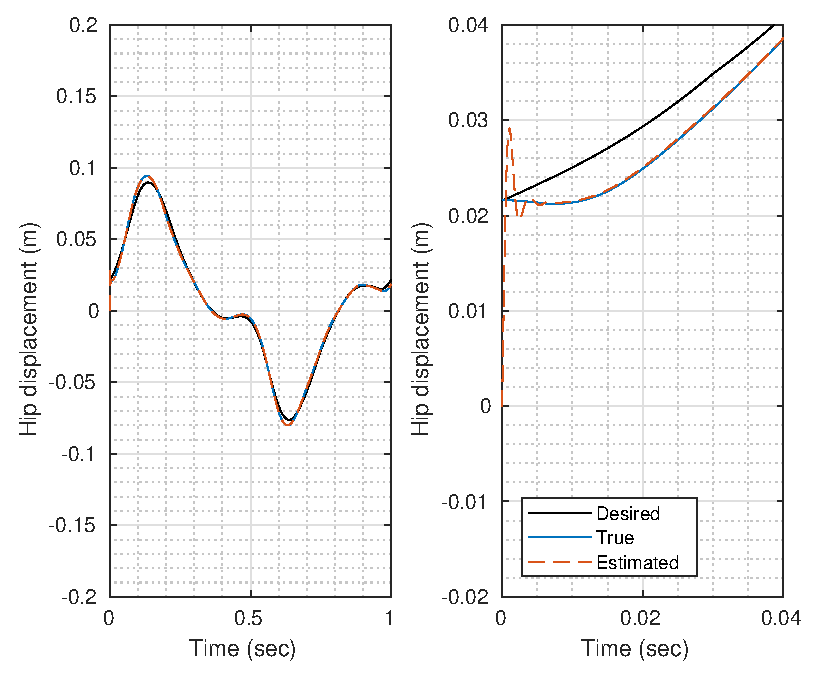
\includegraphics[width = \columnwidth]{Figs/q_hip_mu_1e-03.eps}
	\caption{ Simulation results from a desired hip movement, the controlled plant state and the estimated state from the HGO with constant parameter $\mu=0.001$. The right plot shows the signals behaviours until the first 40ms of simulation}
	\label{fig:hip}
	\end{center}
\end{figure}
%
%
\begin{figure}[h!]
	\begin{center}
	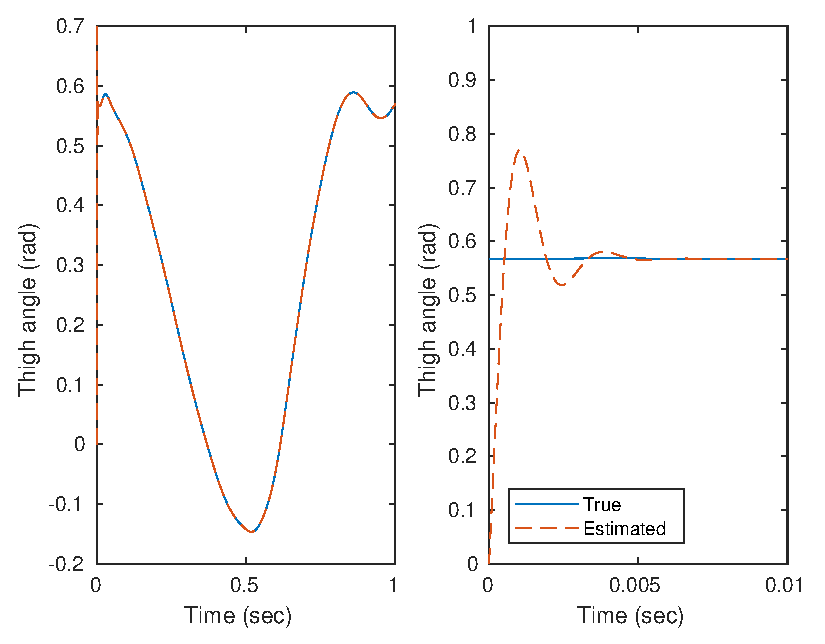
\includegraphics[width = \columnwidth]{Figs/q_thigh_mu_1e-03.eps}
	\caption{ Simulation results from a desired thigh movement, the controlled plant state and the estimated state from the HGO with constant parameter $\mu=0.001$. The right plot shows the signals behaviours until the first 40ms of simulation}
	\label{fig:thigh}
	\end{center}
\end{figure}
%
%
\begin{figure}[h!]
	\begin{center}
	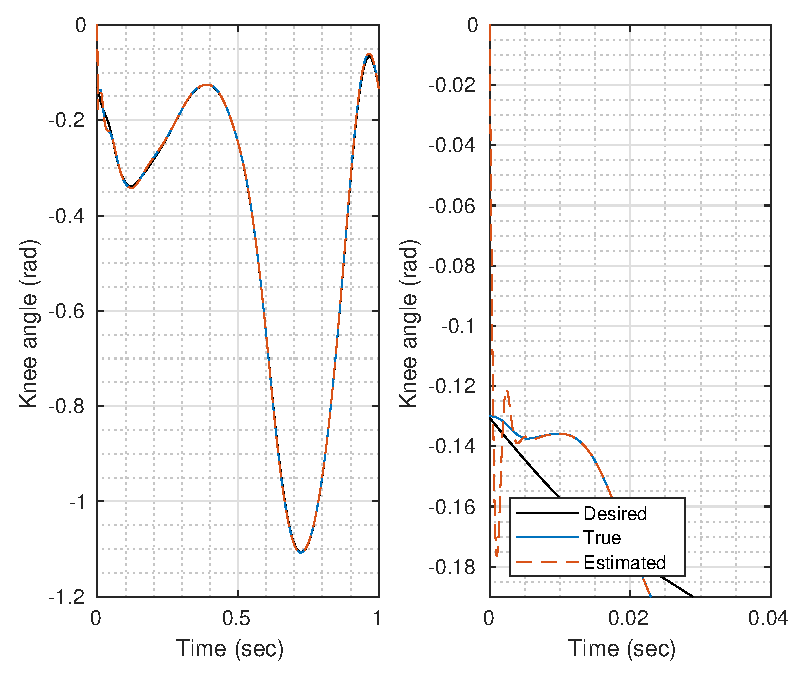
\includegraphics[width = \columnwidth]{Figs/q_knee_mu_1e-03.eps}
	\caption{ Simulation results from a desired knee movement, the controlled plant state and the estimated state from the HGO with constant parameter $\mu=0.001$. The right plot shows the signals behaviours until the first 40ms of simulation}
	\label{fig:knee}
	\end{center}
\end{figure}
%
%
\begin{figure}[h!]
	\begin{center}
	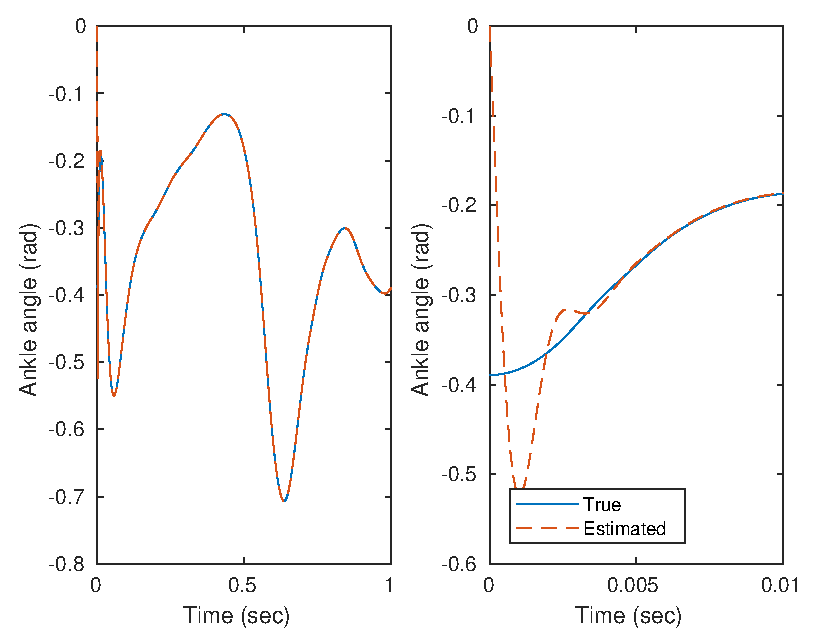
\includegraphics[width = \columnwidth]{Figs/q_ankle_mu_1e-03.eps}
	\caption{ Simulation results from a desired ankle movement, the controlled plant state and the estimated state from the HGO with constant parameter $\mu=0.001$. The right plot shows the signals behaviours until the first 40ms of simulation}
	\label{fig:ankle}
	\end{center}
\end{figure}
%
%
% Velocity plots
%
%
The corresponding hip, thigh, knee and ankle velocities are illustrated in Fig.~\ref{fig:dhip}, Fig.~\ref{fig:dthigh}, Fig.~\ref{fig:dknee} and Fig.~\ref{fig:dankle}, respectively. The RMSE for tracking error in Table.~\ref{table:RMSE_track} shows that velocities in knee and ankle joints require a faster control law to track. That happens because of higher frequency components which also contribute to a worst state estimation in HGO.
%
%
\begin{figure}[h!]
	\begin{center}
	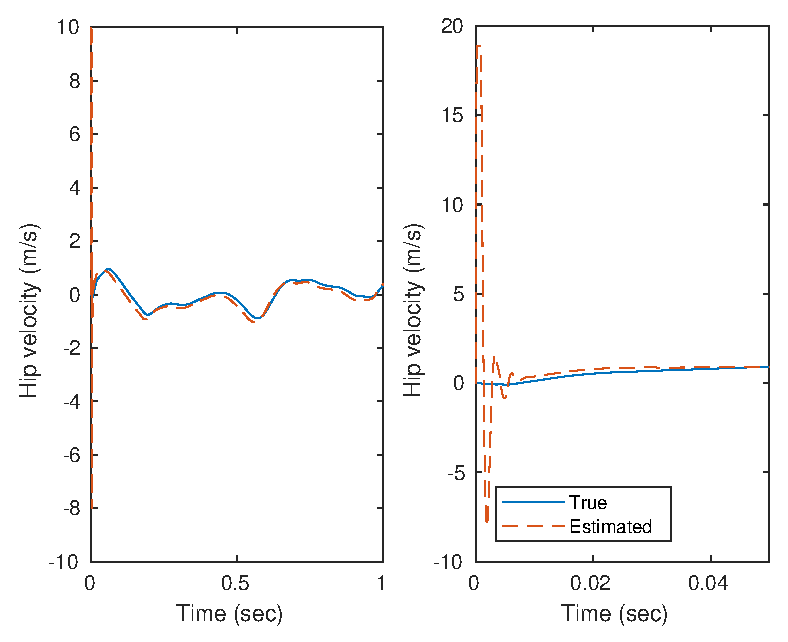
\includegraphics[width = \columnwidth]{Figs/dq_hip_mu_1e-03.eps}
	\caption{ Simulation results from a desired hip velocity, the controlled plant state and the estimated state from the HGO with constant parameter $\mu=0.001$. The right plot shows the signals behaviours until the first 15ms of simulation.}
	\label{fig:dhip}
	\end{center}
\end{figure}
%
%
\begin{figure}[h!]
	\begin{center}
	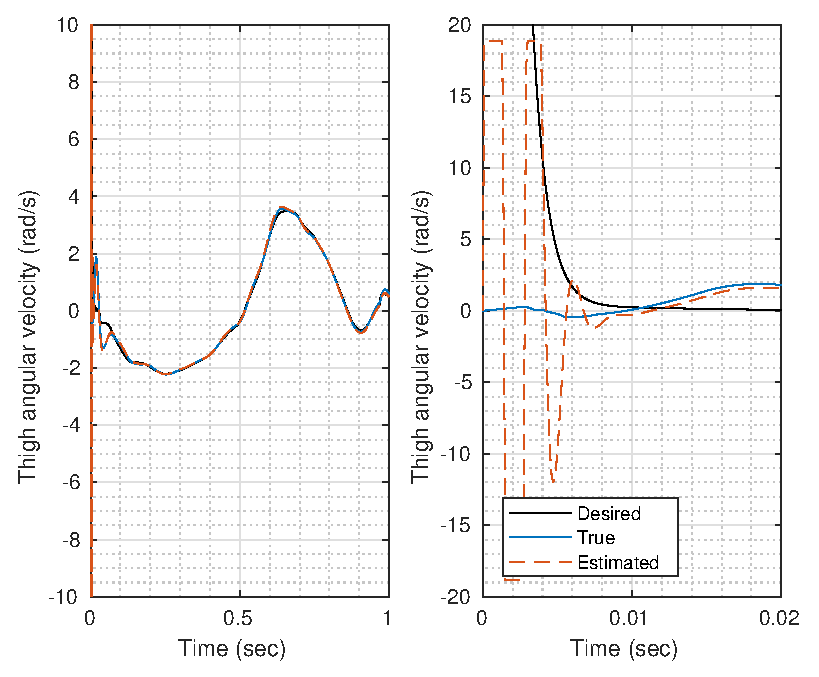
\includegraphics[width = \columnwidth]{Figs/dq_thigh_mu_1e-03.eps}
	\caption{Simulation results from a desired thigh velocity, the controlled plant state and the estimated state from the HGO with constant parameter $\mu=0.001$. The right plot shows the signals behaviours until the first 15ms of simulation.}
	\label{fig:dthigh}
	\end{center}
\end{figure}
%
%
\begin{figure}[h!]
	\begin{center}
	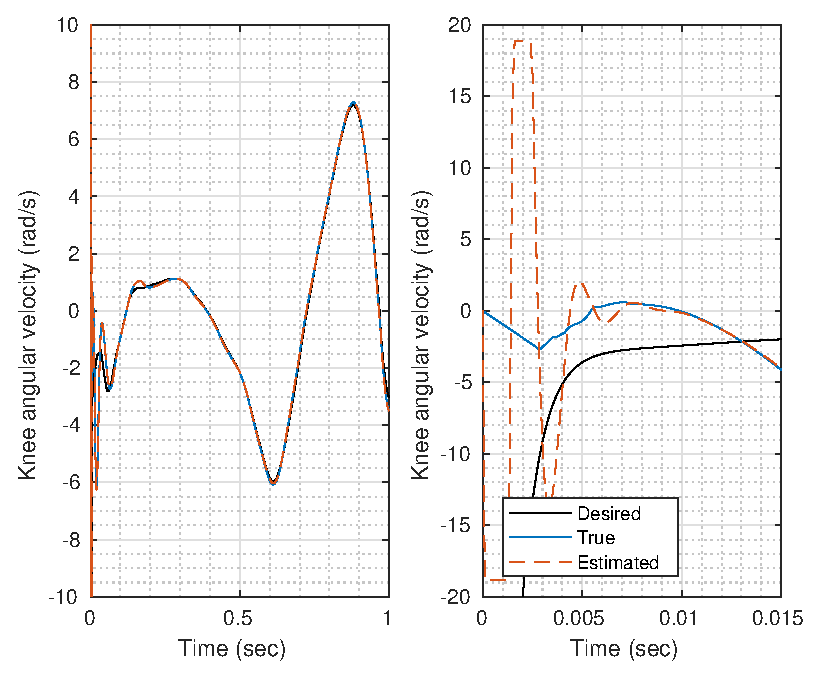
\includegraphics[width = \columnwidth]{Figs/dq_knee_mu_1e-03.eps}
	\caption{Simulation results from a desired knee velocity, the controlled plant state and the estimated state from the HGO with constant parameter $\mu=0.001$. The right plot shows the signals behaviours until the first 15ms of simulation.}
	\label{fig:dknee}
	\end{center}
\end{figure}
%
%
\begin{figure}[h!]
	\begin{center}
	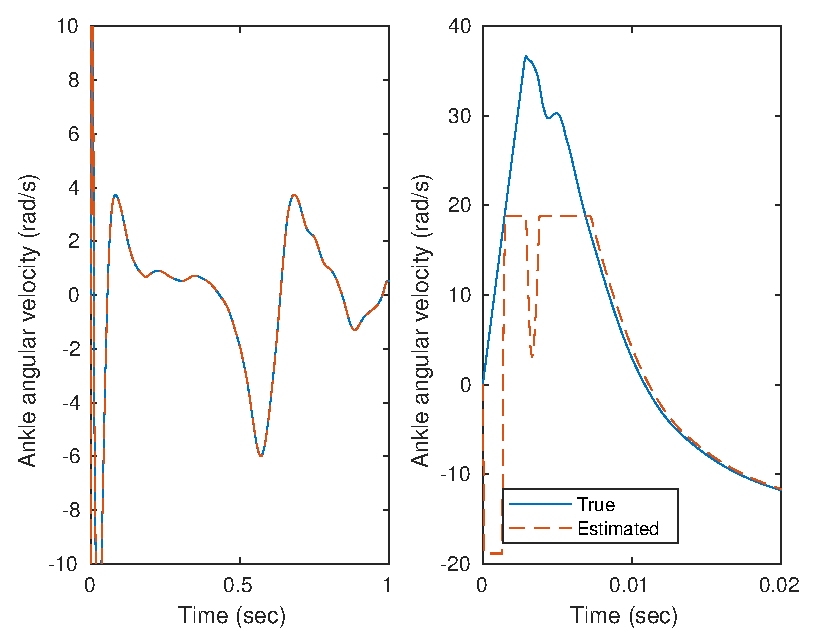
\includegraphics[width = \columnwidth]{Figs/dq_ankle_mu_1e-03.eps}
	\caption{Simulation results from a desired ankle velocity, the controlled plant state and the estimated state from the HGO with constant parameter $\mu=0.001$. The right plot shows the signals behaviours until the first 15ms of simulation.}
	\label{fig:dankle}
	\end{center}
\end{figure}
%
%
Now, in order to illustrate one possible scenario in which the time-varying HGO parameter can be used, the plant parameters are known with parametric error. In order to observe the effect of the input disturbance, a large but unknown constant input disturbance is employed during the whole simulation. 

There is an integral action implemented in the control scheme, therefore the input disturbance causes a transient in the tracking error and any steady state error will be compensated. This transient increases as $\mu$ increases and it is useful to illustrate the usage of the time-varying parameter $\mu$.


By applying a constant value of $\mu(t)= 1.9e-3$ an apparent degradation in the closed-loop tracking error transient is observed in Fig.~\ref{fig:timevarying1}~(a). On the other hand, the noise amplitude in the control signal is acceptable as can be observed in Fig.~\ref{fig:timevarying1}~(b) with the corresponding measurement of the noise amplitude illustrated in Fig.~\ref{fig:timevarying1}~(c). The noise amplitude was obtained by filtering the control input $u$ with a high-pass filter. 
%

%
By reducing $\mu$ to the constant small value $\mu(t)=4e-4$, the  tracking error transient is improved in exchange of an increase on the control signal noise, see  Fig.~\ref{fig:timevarying2}~(a), (b) and (c).
%

%
On the other hand, when the time-varying $\mu(t)$ is implemented starting with the same large value for
$\bar{\mu}\!=\!0.1$,
the tracking error transient is improved, see Fig.~\ref{fig:timevarying3}~(a), without reducing $\mu$ to a prohibitive value which can cause a large noise in the control signal, as illustrated in Fig.~\ref{fig:timevarying3}~(b) and (c). 
%

%
In this case, the time
evolution of $\mu(t)$ is shown in Fig.~\ref{fig:timevarying4}~(a), from which one can verify
that $\mu$ reaches a value of $\mu_{var}=1e-3$ depending on the noise power applied  to the system. 
This value is not known {\em a priori}. It is clear that care must be taken while reducing $\bar{\mu}$, since there exists a trade off
between noise reduction and tracking accuracy.
%
%

%
%
\begin{figure}[h!]
	\begin{center}
	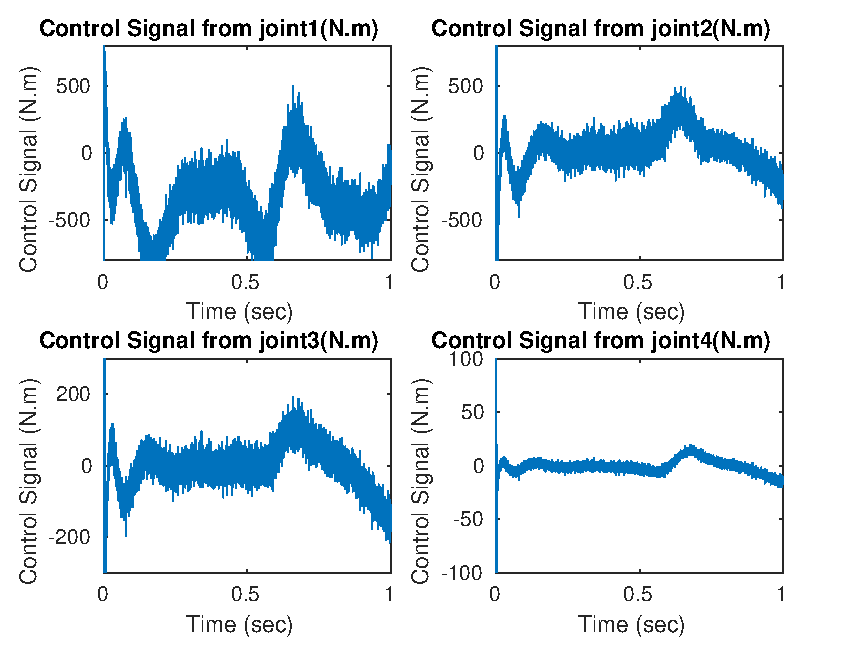
\includegraphics[width = \columnwidth]{Figs/u_mu_fix_4e-04.eps}
	\caption{Simulation results. $\mu = 4e-04$.}
	\label{fig:timevarying4}
	\end{center}
\end{figure}
	%
%
%
\begin{figure}[h!]
	\begin{center}
	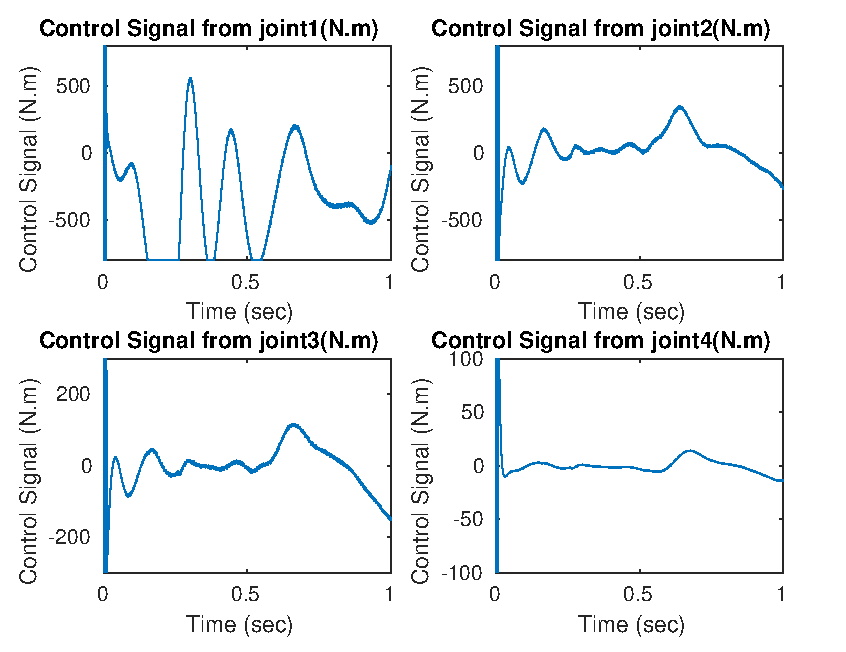
\includegraphics[width = \columnwidth]{Figs/u_mu_fix_2e-03.eps}
	\caption{Simulation results. $\mu = 19e-04$.}
	\label{fig:timevarying4}
	\end{center}
\end{figure}
	%
%
\begin{table}[]
	\centering
	\caption{Tracking root-mean-square-error (RMSE) of a human gait for each joint of a prosthetic leg with estimated states according to the observer gain $\mu$}
	\resizebox{\columnwidth}{!}{%
	\begin{tabular}{ccccccccc}
	\hline
	$\mu$      & $x_1$ (m) & $x_2$ (rad) & $x_3$ (rad) & $x_4$ (rad) & $\dot{x}_1$ (m/s) & $\dot{x}_2$ (rad/s) & $\dot{x}_3$ (rad/s) & $\dot{x}_4$ (rad/s) \\ \hline
	0.4e-3   & 0.0004 & 0.0002 & 0.0009  & 0.0004  & 0.0159  & 0.0117    &  0.0959   &  0.0492   \\
	1.9e-3   & 0.0035 & 0.0013 & 0.0033  & 0.0062  & 0.1120  & 0.0587    &  0.2405   &  0.6836   \\
	Variable & 0.0008 & 0.0004 & 0.0025  & 0.0059  & 0.0257  & 0.0375    &  0.2268   &  0.6640
	\end{tabular}
	\label{table:RMSE_track}
	}%
\end{table}

\begin{table}[]
	\centering
	\caption{Estimation root-mean-square-error (RMSE) of a human gait for each joint of a prosthetic leg with estimated states according to the observer gain $\mu$}
	\resizebox{\columnwidth}{!}{%
	\begin{tabular}{ccccccccc}
	\hline
	$\mu$      & $x_1$ (m) & $x_2$ (rad) & $x_3$ (rad) & $x_4$ (rad) & $\dot{x}_1$ (m/s) & $\dot{x}_2$ (rad/s) & $\dot{x}_3$ (rad/s) & $\dot{x}_4$ (rad/s) \\ \hline
	0.4e-3   & 0.0001 & 0.0036 & 0.0008  & 0.0024  & 0.2607  & 0.4228    &  0.3570   &  0.4065   \\
	1.9e-3   & 0.0004 & 0.0065 & 0.0015  & 0.0045  & 0.3973  & 0.7754    &  0.5952   &  0.8514   \\
	Variable & 0.0003 & 0.0065 & 0.0015  & 0.0045  & 0.3167  & 0.7724    &  0.5948   &  0.8512
	\end{tabular}
	\label{table:RMSE_est}
	}%
\end{table}

%%%%%%%%%%%%%%%%%%%%%%%%%%%%%%%%%%%%%%%%%%%%%%%%%%%%%%%%%%%%%%%%%%%%%%%%%%%%%%%%
\section{Conclusions and Future Work}
\label{sec:Conclusions}
%\subsection{Conclusions}

In this note, we considered the state estimation problem of a robot/prosthesis control system with vertical hip displacement, thigh angle and knee angle.  It was verified that it is possible to apply HGO with dynamic gain in order to reduce the amount of noise in the control signal while assuring an reasonable output tracking error transient. Moreover, when a norm observer is available, domination techniques can be used to design the HGO dynamic gain to obtain global/semi-global practical tracking. An illustrative academic simulation example was presented.


Future possible topics of research are: (i) consider the full robot/prosthesis model including the ground reaction forces and the ankle joint and its estimation; (ii) verify if it is possible to obtain a norm bound for the system state in order to assure global/semi-global stability properties; (iii) design and implementation of the smooth sliding control scheme and (iv) perform experimental results.

%%%%%%%%%%%%%%%%%%%%%%%%%%%%%%%%%%%%%%%%%%%%%%%%%%%%%%%%%%%%%%%%%%%%%%%%
\begin{footnotesize}
%%%
\end{footnotesize}
\bibliography{IEEEabrv,BibProtese,TVHGO} 
%
%\bibliographystyle{unsrt}
%\bibliography{BibProtese}
%


%===============================================================

\appendix


\subsection{System Matrices and Parameters}\label{ap:system}


The plant parameters are given in Table~\ref{table:actual}, while the matrices $D(q), C(q,\dot{q})$ and $g(q)$, appearing in (\ref{eq:Dinamica}), are given by:
%
\begin{eqnarray}
C(1,1) &=&  C(2,1) = C(3,1)=C(3,3)=0\,, \nonumber\\
C(1,2) & =& -\dot{q_2}(L_2m_3+m_2(C_2+L_2)) \sin(q_2)-C_3m_3(\dot{q_2}+\dot{q_3}) \sin(q_2+q_3)\,, \nonumber\\
C(1,3) &=&  -C_3 m_3 \sin(q_2+q_3)(\dot{q_2}+\dot{q_3})\,, \nonumber\\
C(2,2) &=&  -C_3 L_2 m_3\dot{q_3} \sin(q3)\,, \nonumber\\
C(2,3) &=&  -C_3 L_2 m_3 \sin(q_3)(\dot{q_2}+\dot{q_3})\,, \nonumber\\
C(3,2) &=&  C_3 L_2 m_3\dot{q_2} \sin(q_3)\,,\label{eq:defC}
\end{eqnarray}
%
%
\begin{eqnarray}
D(1,1) &=& m_1 + m_2 + m_3 \,, \nonumber \\
D(1,2) &=& D(2,1) = (c_3 \cos(q_2+q_3) + l_2 \cos(q_2)) + m_2 (c_2 \cos(q_2) + l_2 \cos (q_2) )\,, \nonumber \\
D(1,3) &=& D(3,1) = c_3 m_3 \cos( q_2 + q_3) \,, \nonumber \\
D(2,2) &=& I_{2z} + I_{3z} + c_2^2 m_2 + c_3^2 m_3 + I_2^2 (m_2 + m_3) + 2 c_2 l_2 m_2 + 2 c_3 l_2 m_3 \cos (q_3)\,, \nonumber\\
D(2,3) &=& D(3,2) m_3 c_3^2 + l_2 m_3 \cos (q_3 ) c_3 + I_{3z} \,,\nonumber \\
D(3,3) &=&  m_3 c_3^2 + I_{3z}\,,\label{eq:defD}
\end{eqnarray}
%
\begin{eqnarray}
g(1,1) &=&  -g(m_1+m_2+m_3)\,, \nonumber\\
g(2,1) &=&  -C_3 g m_3 \cos(q_2+q_3)-g (m_2(C_2+L_2)+L_2 m_3) \cos(q_2)\,, \nonumber\\
g(3,1) &=&  -C_3 g m_3 \cos(q_2+q_3)\,.
\label{eq:defg}
\end{eqnarray}
%
% Updated value
%
\begin{eqnarray}
	D(1,1) &=& \Theta_1\nonumber\\
	D(1,2) &=& \Theta_{2}cos(q_{2}) + \Theta_{3}cos(q_{2} + q_{3} + q_{4}) + \Theta_{4}cos(q_{2} + q_{3})\nonumber\\
	D(1,3) &=& \Theta_{3}cos(q_{2} + q_{3} + q_{4}) + \Theta_{4}cos(q_{2} + q_{3})\nonumber\\
	D(1,4) &=& \Theta_{3}cos(q_{2} + q_{3} + q_{4}) \nonumber \\
	D(2,1) &=& D(1,2)\nonumber \\
	D(2,2) &=& \Theta_{5} + 2\Theta_{6}cos(q_{3} + q_{4}) + 2\Theta_{7}cos(q_{3}) + 2\Theta_{8}cos(q_{4})\nonumber \\
	D(2,3) &=& \Theta_{9} + \Theta_{7}cos(q_{3}) + 2\Theta_{8}cos(q_{4}) + \Theta_{6}cos(q_{3} + q_{4})\nonumber \\
	D(2,4) &=& \Theta_{10} + \Theta_{6}cos(q_{3} + q_{4}) + \Theta_{8}cos(q_{4}) \nonumber \\
	D(3,1) &=& D(1,3)\nonumber \\
	D(3,2) &=& D(2,3)\nonumber \\
	D(3,3) &=& \Theta_{9} + 2\Theta_{8}cos(q_{4}) + m_{4}l_{3}^2 + I_{3z} + I_{4z} \nonumber \\
	D(3,2) &=& \Theta_{10} + \Theta{8}cos(q_{4}) \nonumber \\
	D(4,1) &=& D(1,4)\nonumber \\
	D(4,2) &=& D(2,4)\nonumber \\
	D(4,3) &=& D(3,4)\nonumber \\
	D(4,4) &=& \Theta_{10} \nonumber \\
	\label{eq:Inertia}
\end{eqnarray}
%
%
\begin{eqnarray}
	C(1,1) &=& 0\nonumber\\
	C(1,2) &=& - \dot{q_{3}}(\Theta_{3}sin((q_{2} + q_{3} + q_{4}) + \Theta_{4}sin(q_{2} + q_{3})) - \dot{q_{2}}(\Theta_{2}sin(q_{2}) + \Theta_{3}sin((q_{2} + q_{3} + q_{4}) + \Theta_{4}sin(q_{2} + q_{3})) - \Theta_{3}\dot{q_{4}}sin(q_{2}+ q_{3}+ q_{4}) \nonumber\\
	C(1,3) &=& \dot{q_{2}}(\Theta_{3}sin((q_{2} + q_{3} + q_{4}) + \Theta_{4}sin(q_{2} + q_{3})) - \dot{q_{3}}(\Theta_{3}sin((q_{2} + q_{3} + q_{4}) + \Theta_{4}sin(q_{2} + q_{3})) - \Theta_{3}\dot{q_{4}}sin(q_{2}+ q_{3}+ q_{4}) \nonumber\\
	C(1,4) &=& \Theta_{3}\dot{q_{2}}sin(q_{2}+ q_{3}+ q_{4}) - \Theta_{3}\dot{q_{3}}sin(q_{2}+ q_{3}+ q_{4}) - \Theta_{3}\dot{q_{4}}sin(q_{2}+ q_{3}+ q_{4}) \nonumber \\
	C(2,1) &=& 0 \nonumber \\
	C(2,2) &=& - \dot{q_{3}}(\Theta_{6}sin(q_{3} + q_{4}) + \Theta_{7}sin(q_{3})) - \dot{q_{4}}(\Theta_{6}sin(q_{3} + q_{4}) + \Theta_{8}sin(q_{4})) \nonumber \\
	C(2,3) &=& 0 \nonumber \\
	C(2,4) &=& 0 \nonumber \\
	C(3,1) &=& 0 \nonumber \\
	C(3,2) &=& 0 \nonumber \\
	C(3,3) &=& 0 \nonumber \\
	C(3,2) &=& 0 \nonumber \\
	C(4,1) &=& 0 \nonumber \\
	C(4,2) &=& 0 \nonumber \\
	C(4,3) &=& 0 \nonumber \\
	C(4,4) &=& 0 \nonumber \\
	\label{eq:Coriolis}
\end{eqnarray}
%
%
\begin{table}[h!]
\centering
\caption{Plant parameters table}
\begin{tabular}{ |p{3cm} p{3cm} p{3cm}|  }
 \hline
 %\multicolumn{4}{|c|}{Plant parameters} \\
 %\hline
 Parameter & Value & Units\\
 \hline
	$m_1$ & 21.29 & $Kg$\\
	$m_2$ & 8.57 & $Kg$\\
	$m_3$ & 2.33 & $Kg$\\
	$I_2$ & 0.435 & $Kg-m^2$\\
	$I_3$ & 0.062 & $Kg-m^2$\\
	$d_0$ & 0.5 & $m$ \\
	$L_2$ & 0.425 & $m$ \\
	$L_3$ & 0.527 & $m$ \\
	$C_2$ & -0.339 & $m$ \\
	$C_3$ & 0.320 & $m$ \\
	$g$ & 9.81 & $m/s^2$ \\
\hline
\end{tabular}
\label{table:actual} 
\end{table}



\end{document}
%%%%%%%%%%%%%%%%%%% E N D  O F   F I L E %%%%%%%%%%%%%%%%%%%%%%%%%%%%%%%%%%
